% Figura cuerpo B2 (3.1.2): un precio relativo que no responde al exceso de oferta: el desempleo involuntario como equilibrio
\documentclass[tikz,border=3pt]{standalone}
\usepackage[T1]{fontenc}
\usepackage[utf8]{inputenc}
\usepackage{amsmath}
\usetikzlibrary{arrows.meta,calc,positioning}
\begin{document}
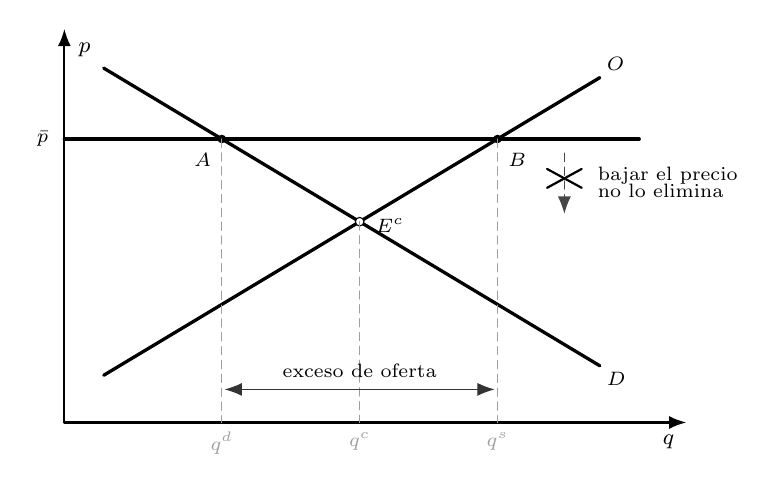
\begin{tikzpicture}[>={Latex[length=2.2mm]}, line cap=round, font=\footnotesize,
  eje/.style={->, thick},
  curva/.style={very thick},
  guia/.style={densely dashed, gray!75},
  pto/.style={circle, fill=black, inner sep=1.1pt},
  contra/.style={circle, draw=black, fill=white, inner sep=1.1pt}]

  \draw[eje] (0,0) -- (7.9,0) node[below left=1pt]{$q$};
  \draw[eje] (0,0) -- (0,5.0) node[below right=2pt]{$p$};

  % Demanda y oferta
  \draw[curva] (0.5,4.5) -- (6.8,0.72) node[below right=-2pt, font=\scriptsize]{$D$};
  \draw[curva] (0.5,0.6) -- (6.8,4.38) node[above right=-2pt, font=\scriptsize]{$O$};

  % Precio relativo deseado, rígido
  \draw[very thick] (0,3.6) -- (7.3,3.6);
  \node[anchor=east, font=\scriptsize] at (-0.08,3.6) {$\bar{p}$};

  % Vaciado que no ocurre
  \node[contra] (Ec) at (3.75,2.55) {};
  \node[anchor=west, inner sep=2pt, font=\scriptsize] at (3.88,2.50) {$E^{c}$};
  \draw[guia] (3.75,2.55) -- (3.75,0) node[below, font=\scriptsize]{$q^{c}$};

  % Las dos cantidades al precio rígido
  \node[pto] (A) at (2.0,3.6) {};
  \node[anchor=north east, inner sep=2pt, font=\scriptsize] at (1.94,3.50) {$A$};
  \node[pto] (B) at (5.5,3.6) {};
  \node[anchor=north west, inner sep=2pt, font=\scriptsize] at (5.56,3.50) {$B$};
  \draw[guia] (2.0,3.6) -- (2.0,0) node[below, font=\scriptsize]{$q^{d}$};
  \draw[guia] (5.5,3.6) -- (5.5,0) node[below, font=\scriptsize]{$q^{s}$};
  \draw[<->, gray!40!black, shorten >=1pt, shorten <=1pt] (2.0,0.42) -- (5.5,0.42);
  \node[anchor=south, font=\scriptsize] at (3.75,0.45) {exceso de oferta};

  % El ajuste a la baja que no se produce
  \draw[->, gray!55!black, densely dashed] (6.35,3.42) -- (6.35,2.65);
  \draw[thick] (6.13,3.22) -- (6.57,2.98);
  \draw[thick] (6.13,2.98) -- (6.57,3.22);
  \node[anchor=west, font=\scriptsize, align=left] at (6.65,3.05) {bajar el precio\\[-2pt]no lo elimina};

\end{tikzpicture}
\end{document}
